\newpage
\chapter*{ANN-Marco Lourenço}

\section*{Introduction}

Le but de ce challenge était de choisir entre plusieurs algorithmes de Machine Learning afin de tenter de réaliser le score le plus élevé avec un DataSet fourni comprenant des mouvements enregistrés à l'aide d'une Kinect (sous-dataset skeleton) ou avec un capteur Xsens (sous-dataset xsens). Le programme pouvait être implémenté en Matlab ou C\#.\\

J'ai choisi d'implémenter un "Artificial Neural Network" car je suis un minimum à l'aise avec Matlab et que Matlab est bien équipé pour ce cas-là.

\section*{Preprocessing}

Aucun preprocessing n'a été implémenté pour améliorer les données du dataset.\\

Les preprocessing possibles auraient été le scaling des features ou la standardisation des features. Ces techniques de preprocessing sont utiles car certains algorithmes dont ANN ignorent les features avec une échelle réduite.

\section*{Extraction des features}

Afin de pouvoir entraîner le réseau de neurones, il est nécessaire au préalable d'extraire du dataset les features qui représentent au mieux les mouvements et les gestes. Les gestes sont répartis en 11 classes distinctes : \\

\begin{itemize}
\item Calibration
\item Swipe left
\item Swipe right
\item Push to screen
\item Take from screen
\item Palm-up rotation
\item Palm-down rotation
\item Draw a circle I
\item Draw a circle II
\item Wave hello
\item Shake hand
\end{itemize}

Néanmoins, avant de pouvoir travailler avec les données, il est nécessaire de comprendre la structure dans laquelle elles sont stockées. Dans notre cas, on peut représenter les informations des capteurs comme ceci :

\begin{figure}[h]
  \centering
    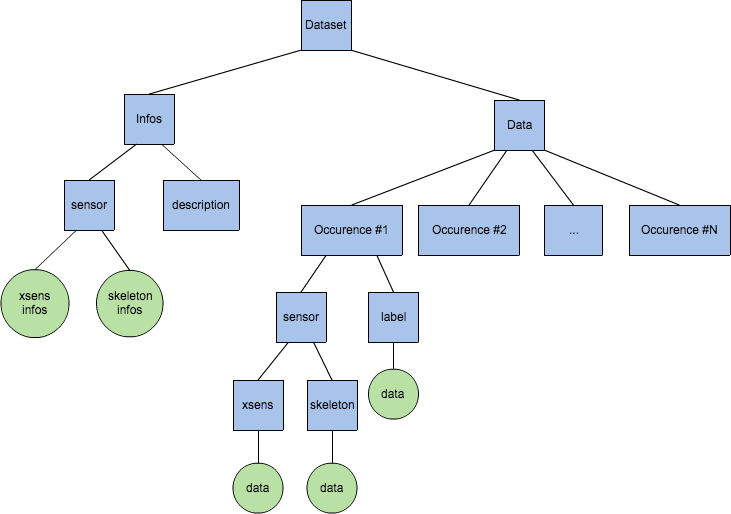
\includegraphics[width=0.8\linewidth]{img/ann/extract/ann_dataset_mpri.png}
  \caption{Structure des données}
  \label{fig:dataset_mpri}
\end{figure}

Les données ne sont pas directement séparées par type de capteur, mais plutôt par occurence. Une occurence représente simplement en d'autres mots une session d'enregistrement d'un mouvement. Chaque occurence est marquée d'un label, qui indique de quel geste on parle (cf. les 11 classes). Cela est nécessaire pour l'apprentissage supervisé. \\

Ensuite, dans chaque occurence, les données sont séparées par type de capteur. Finalement, on accède aux données brutes. Néanmoins, ce n'est pas fini. Si l'on souhaite travailler avec ces données, il est nécessaire de savoir ce qu'elles représentent. Pour cela, direction la section "infos" du dataset, qui permet de savoir ce que chaque colonnes représente. \\

Pour résumé, le sous-dataset skeleton est organisé en articulations (principe de la Kinect). En voici la liste : \\

\begin{itemize}
\item HipCenter 
\item Spine 
\item ShoulderCenter 
\item Head 
\item ShoulderLeft
\item ElbowLeft 
\item WristLeft 
\item HandLeft 
\item ShoulderRight
\item ElbowRight 
\item WristRight 
\item HandRight 
\item HipLeft 
\item KneeLeft
\item AnkleLeft 
\item FootLeft 
\item HipRight 
\item KneeRight 
\item AnkleRight 
\item FootRight
\end{itemize}
\bigskip
Chacune de ces articulations ensuite est sous-divisée en 4 informations : TrackingState X Y Z. Cela donne donc en tout 84 données à traiter. Le même principe général s'applique pour le sous-dataset xsens (différentes données pour chaque différent point sur le corps). \\

Au final donc, les données de skeleton sont organisées en 84 colonnes. Ensuite, chaque ligne représentera un point dans le temps, avec les 84 données associées. Si l'on veut visualiser les points parcourus dans le temps, il est nécessaire de parcourir toutes les lignes. \\

Une fois ces observations effectuées, il est nécessaire de choisir des features. Dans un premier temps, on pourrait simplement garder les données telles quelles afin de créer la matrice qui servira d'input à l'ANN. Néanmoins, il est quand même nécessaire de filtrer un peu. \\

Dans cette optique, j'ai décidé de garder les données de la Kinect uniquement, car je me suis dit que les positions de certains membres du corps étaient largement suffisantes pour décrire assez bien un geste. Ensuite, j'ai décidé de garder les données de la partie haute du corps comme indiqué dans la donnée de l'exercice, car de toute manière les parties du bas ne sont pas exploitées. \\

Le code proposé comme base pour ce projet permettait déjà d'extraire uniquement certaines données (i.e. certaines colonnes) et classait le tout par classe. Il suffisait donc ensuite d'ajuster les colonnes extraites au données voulues (Head, ShoulderLeft, ...) et de parcourir le trainSet ainsi :

\begin{lstlisting}
pour chaque classe
	pour chaque occurence
    		concatener verticalement les donnees "features" du dataset
	end 
end
transposer la matrice 
\end{lstlisting}

Le résultat final est comme on l'espère une matrice avec sur chaque ligne chaque feature choisie (position X de la tête, position Y du coude gauche, ...) et sur chaque colonne les échantillons mesurés. Il faut noter que la notion de temps est conservée dans ce format. Cela est un problème discuté dans la section "Problèmes rencontrés". 

\section*{Entrainement et évaluation}

Une fois les données converties en une matrice utilisable par Matlab, il est nécessaire de mettre en place un réseau de neurone. Pour cela, la toolbox de "Neural Net Pattern Recognition" permet de grandement accéléré le processus en proposant un assistant de création qui va créer pour nous un réseau "feed-forward" à deux couches.

\begin{figure}[h]
  \centering
    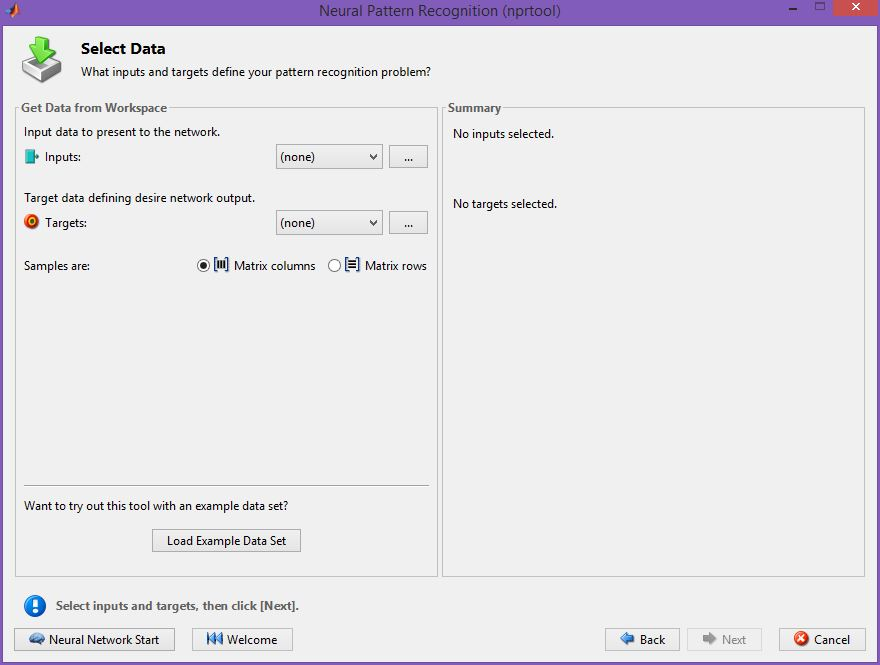
\includegraphics[width=0.8\linewidth]{img/ann/train/ann_toolbox_1.jpg}
  \caption{Choix des données}
  \label{fig:toolbox_1}
\end{figure}

On peut ensuite facilement donner au système les données sur lesquelles il doit s'entraîner (Inputs) mais aussi les données qui lui permettent de vérifier si les résultats sont corrects (Targets). Il est également facile de changer le nombre de neurones dans la couche cachée. Par défaut, le système va utiliser 70\% des données pour s'entraîner, 15\% pour optimiser le modèle et les 15\% restants pour faire les tests et obtenir le résultat final (figure \ref{fig:dataset_split}). \\

Une fois que l'on est satisfait du résultat, on peut simplement demander à la toolbox de générer le code que l'on pourra ensuite introduire dans le code de base du projet. Ici, il est nécessaire de splitter le code entre "TrainModel.m" et "Recognize.m" afin de respecter la structure donnée. Les méthodes principales à retenir sont "net()" et "train()". "net()" est la méthode qui retourne la liste des classes prédites en fonction d'un dataset en input et "train()" est la méthode qui va entraîner pour nous le réseau de neurones avec les paramètres donnés.\\

\begin{figure}[h]
  \centering
    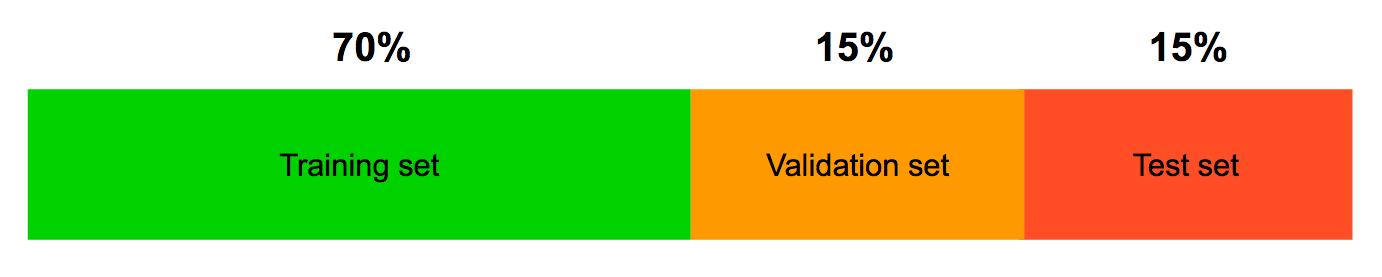
\includegraphics[width=0.8\linewidth]{img/ann/train/ann_repartition.png}
  \caption{Répartition du dataset}
  \label{fig:dataset_split}
\end{figure}

Le seul paramètre ici en notre contrôle est le nombre de neurones de la couche cachée, mais il s'est avéré que le changer n'affectait pas vraiment les résultats. Les pistes pour le modifier sont multiples : on peut tenter de l'incrémenter et de refaire l'entraînement à chaque fois ou alors il est possible de l'adapter à une variable importante de notre problème, par exemple ici 11 pour le nombre de classes. Il est généralement déconseillé d'utiliser des chiffres trop élevés. Le réseau utilisé avec 10 neurones dans la couche cachée est visible dans la figure \ref{fig:network_view}.

\begin{figure}[h]
  \centering
    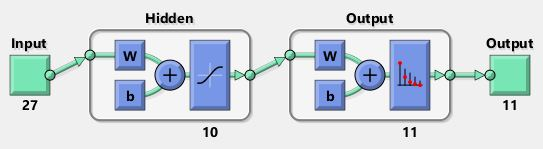
\includegraphics[width=0.8\linewidth]{img/ann/train/network_view.jpg}
  \caption{Réseau de neurones}
  \label{fig:network_view}
\end{figure}

\section*{Résultats}

Les résultats en terme de score sont les suivants :

\begin{center}
\begin{tabularx}{\textwidth}{|X|X|}
\hline 
Precision & 0.463 \\ 
\hline 
Recall & 0.484 \\ 
\hline 
F1 Score (test) & 0.473 \\ 
\hline 
F1 Score (opegra) & 0.672 \\ 
\hline 
\end{tabularx} 
\end{center}

On peut voir que le score sur le dataset d'opegra (figure \ref{fig:opegra}) est meilleur que celui sur le test set, et ce d'une bonne longueur. Les scores en local ont été calculés à partir de la matrice de confusion visible en figure \ref{fig:matrice_confu}. \\

\begin{figure}[h]
  \centering
    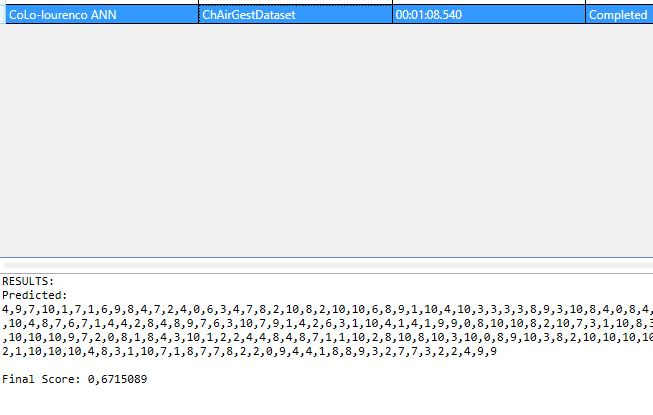
\includegraphics[width=0.8\linewidth]{img/ann/results/opegra.jpg}
  \caption{F1 Score Opegra}
  \label{fig:opegra}
\end{figure}

\begin{figure}[h]
  \centering
    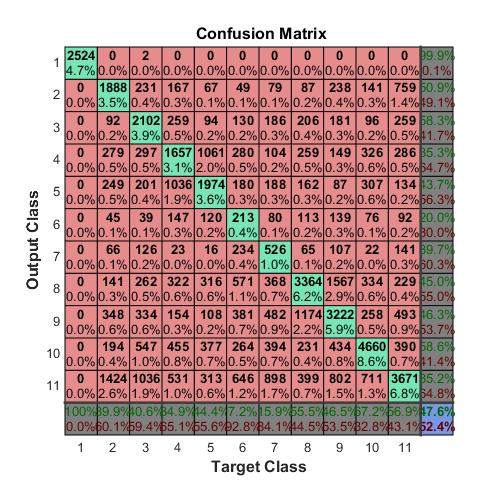
\includegraphics[width=0.8\linewidth]{img/ann/results/matrice_confu.jpg}
  \caption{Matrice de confusion}
  \label{fig:matrice_confu}
\end{figure}

Malheureusement, les scores n'étant pas dans les 90\% et plus, il est difficile d'analyser quelles erreurs entre une classe et une autre était les plus répandues. Néanmoins, on peut quand même noter une confusion prononcée entre les classes 4 et 5, 8 et 9 et finalement 11, 2 et 3. On peut également noter que la calibration (classe 1) a correctement été détectée.\\

On peut également voir dans la courbe ROC (figure \ref{fig:roc}) que la détection de certaines classes est bien meilleure que d'autres (la meilleure étant la 1 bien sûr). On peut également voir que malgré le score peu élevé, cette détection reste meilleure qu'une détection aléatoire, symbolisée par la diagonale. Le cas extrême où les courbes sont sous la diagonale est également absent (heureusement). Bien évidemment, ce n'est quand même pas utilisable dans le cadre d'un produit réel.

\begin{figure}[h]
  \centering
    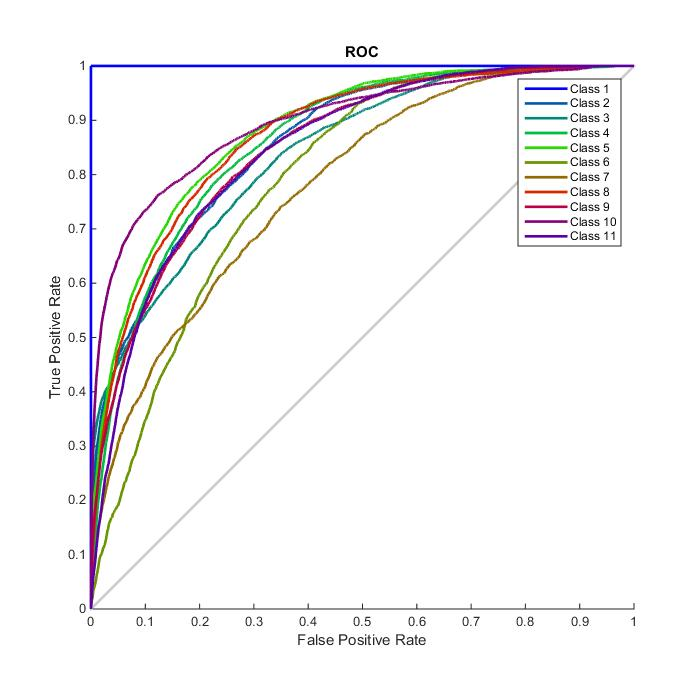
\includegraphics[width=0.8\linewidth]{img/ann/results/ROC.jpg}
  \caption{Courbe ROC}
  \label{fig:roc}
\end{figure}

\section*{Problèmes rencontrés}

Le plus gros problème rencontré pour arriver à ces résultats a été le décryptage du dataset d'entrée. En effet, en ouvrant la structure avec Matlab, cette dernière n'apparait pas aussi clairement que dans le schéma de la figure \ref{fig:dataset_mpri}. Lorsqu'on ouvre la structure occurrence, on a l'impression de voir une liste de senseurs, alors qu'on voit une liste d'occurrences avec pour chacune d'entre elle des senseurs. Cela a mené à une incompréhension du fait d'avoir 861 senseurs. \\

Ce problème vient certainement du fait que dans les TPs, la matrice d'inputs était pour le cas du cosinus un simple vecteur et dans le cas de la détection de voix, les features étaient extraites et disponibles pour la toolbox sans autre effort. Ici, il est nécessaire de bien comprendre la structure du dataset, dans quel format la toolbox veut la matrice, etc ... \\

Un autre problème rencontré a été le fait de ne pas communiquer avec mes collègues. En effet, même si cela semble normal de travailler pour soit étant donné qu'on travaille avec son propre algorithme et qu'aucune tache n'est partageable dans le groupe hormis la présentation, cela m'a conduit à ne pas du tout pensé à la FFT pour l'extraction de features. Cela a considérablement limité les choix d'optimisation étant donné que changer les colonnes extraites ou le nombre de neurones ne changeait pas grand chose dans le résultat obtenu. \\

Tout cela a mené à un mismatch entre le nombre de classes prédites et le nombre d'occurences. En effet, dans la logique et après avoir eu le temps d'y repenser, chaque occurence est un mouvement/geste composé de plusieurs points dans le temps et est représenter par une unique classe. Dans mon cas, chaque occurence avait plusieurs classes prédites, ce qui est maintenant évidemment complètement illogique. Arrivé à ce point-là, tout était mélangé et il était difficile de comprendre pourquoi les tailles ne correspondaient pas. Avec la FFT, chaque occurence aurait bien gardé 1 seule classe prédite et aucun souci ne serait arrivé.

\section*{Améliorations}

La principale amélioration pour ce réseau de neurones est clairement l'ajout de la FFT. Même en ne gardant que la Kinect et en filtrant correctement les données, il est certainement possible d'atteindre des scores très corrects. De plus, il existe de nombreuses autres opérations qu'on peut encore appliquer après la FFT. Tout cela permet d'atteindre des scores très élevés, comme l'ont montrées les présentations.\\

Finalement, il serait judicieux également de tester l'apport de preprocessing sur les données, ainsi qu'un test poussé sur l'incidence qu'a le changement du nombre de neurones de la couche cachée.

\section*{Conclusion}

Malgré le score peu élevé qu'a obtenu mon ANN, je dirais qu'en considérant ce qu'il est possible de faire avec la FFT, un score de 0.67 est déjà vraiment incroyable. Cela veut dire que même si chaque point d'un mouvement est indépendant vis-à-vis du réseau, ce dernier est quand même capable de discerner des patterns et d'effectuer une grande partie des reconnaissances correctement. \\

Si cela montre une chose, c'est bien la puissance du Machine Learning et il n'est donc pas étonnant de savoir que tous les grands acteurs de la Silicon Valley l'ont depuis longtemps intégré dans leurs produits.
 
 
 

